\section{Software}

O escopo geral do projeto é a construção de um sistema para auxiliar usuários no lançamento e monitoramento de foguetes experimentais. O auxílio ao usuário será dado em dois momentos:  

\begin{enumerate}
    \item Abastecimento e Ignição do foguete. 
    \item Foguete em voo.
\end{enumerate}

Para o momento 1, o objetivo é prover uma interface onde o usuário possa realizar comandos para o abastecimento e ignição de um foguete, além de acompanhar os dados de abastecimento em tempo de execução. Esta interface deve ser de fácil entendimento e amigável. O usuário deverá receber confirmações para caso seus comandos tenham sido executados corretamente, ou avisos de erros para caso aconteça problemas.  

Para o momento 2, o objetivo é criar uma interface que promova um ambiente onde o usuário possa fazer o acompanhamento do voo de um foguete. As informações que serão mostradas em telas serão providas por sensores acoplados ao foguete. As informações obtidas também serão persistidas e indexadas em bases de dados e disponibilizadas para consulta e motores de análise. 

Também é o objetivo deste projeto a análise cognitiva de dados históricos e dados obtidos durante os lançamentos, já realizados com nosso sistema. Propomos fazer análises de anomalias durante o voo do foguete, tendo como base e rótulo o sucesso ou não de lançamento anteriores.

\subsection{Representação da arquitetura}

\subsubsection{Visão Geral}
\begin{figure}[H]
\centering
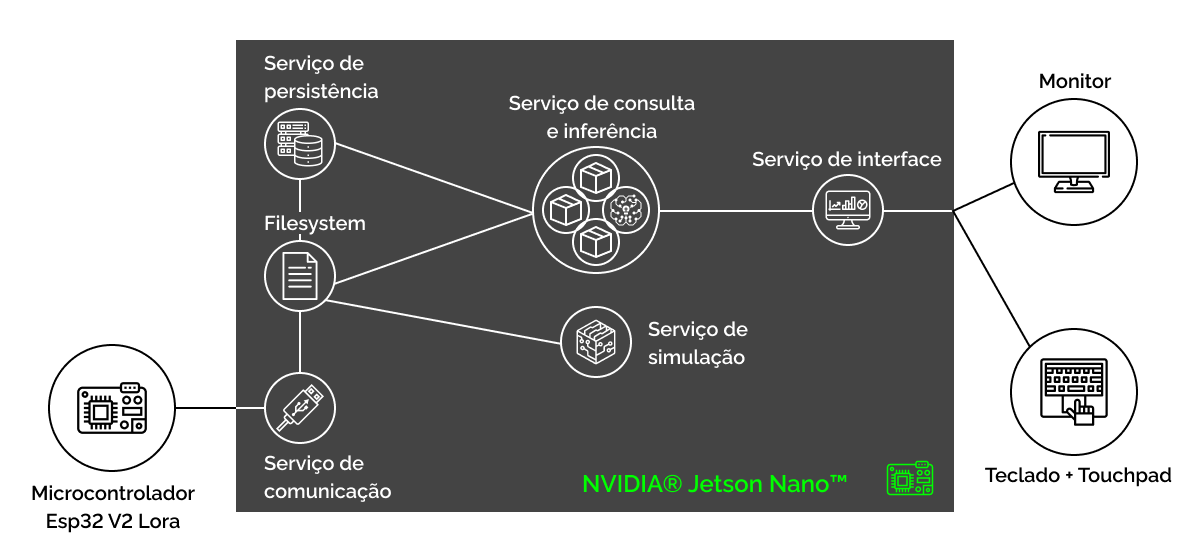
\includegraphics[width=1\textwidth]{figuras/arquitetura_visao_geral}
\caption{Visão geral da arquitetura de software}
\end{figure}

\subsubsection{Serviços}
A arquitetura é baseada no padrão arquitetural \textit{Service oriented architeture}\footnote{Do inglês Service-Oriented Architecture, também conhecido como Arquitetura orientada a serviços.\cite{bieberstein2006service}} (SOA). Esse padrão arquitetural tem suas vantagens devido ao baixo acoplamento entre os módulos e a facilidade de manutenção.

\subsubsubsection{Comunicação}
Esse serviço é responsável por fazer a comunicação do microcontrolador, fazendo escritas e leituras em um \textit{Filesystem}\footnote{Sistema de gerenciamento de arquivos do sistema operacional}. Esse serviço não vai ser usado oficialmente pois não teremos comunicação com o microcontrolador.


\subsubsubsection{Persistência}
Esse serviço trata-se propriamente do banco de dados que será utilizado pelo sistema. Sua função é a indexação e persistência de dados provenientes do acompanhamento do voo de foguetes, bem como a disponibilização desses dados para outras partes do sistema.

\subsubsubsection{Consulta e inferência}
Esse serviço é responsável pelo grande processamento e gerência dos dados, assim como a aplicação de regras negociais específicas. Deverá ser capaz de:
\begin{itemize}
    \item Armazenar e indexar dados obtidos
    \item Disponibilizar dados obtidos em tempo de execução \textit{(streaming)}, para as camada de comunicação com o usuário
    \item Realizar a análise sob os dados obtidos a partir de modelos de ML\footnote{Sigla para  o nome em inglês Machine Learning, ou no portugues aprendizado de máquina.} pré treinados, e fornecer inferência sobre esses dados em tempo de execução
    \item Exportação dos dados
\end{itemize}

\subsubsubsection{Interface}
Esse serviço é responsável pela construção da camada de comunicação com o usuário.

\subsubsubsection{Simulação}
Este serviço é responsável por fazer a simulação da comunicação do microcontrolador, fazendo escritas e leituras em um \textit{Filesystem}. Ele faz-se necessário, pois não teremos integração direta com a microcontrolador.

\subsubsection{Arquitetura computacional}
O sistema será desenvolvido para ser executado em um computador de arquitetura 64 bit ARM (Arm64) e um sistema operacional que opere nessa mesma arquitetura. \cite{arquitetura_arm}

\subsection{Visão de implementação}
\subsubsection{Ambiente}
Tendo em vista a arquitetura orientada a serviço e a falta da placa para testar o sistema nas condições reais, foi adotada a estratégia de conteinerização dos serviços. Assim é possível isolar os ambientes, bem como facilitar a configuração do ambiente de produção (já embarcado no dispositivo). Para isso, foi utilizado as seguintes tecnologias:

\begin{itemize}
    \item Docker \cite{docker}
    \item Docker - Compose \cite{docker-compose}
\end{itemize}


\subsubsection{Machine Learning}
Devido à natureza de algumas características do sistema, principalmente no que diz respeito às funcionalidades que envolvem a utilização de modelos de ML, foi adotado um segundo ambiente de desenvolvimento especialmente voltado para a análise exploratória dos dados, construção e treinamento de modelos de ML. Para isso, utilizaremos as seguintes tecnologias:

\begin{itemize}
    \item Jupyter Notebook \cite{jupyter-notebook}
    \item Tensor Flow \cite{tensorflow}
    \item Keras \cite{keras}
    \item SKlearn \cite{scikit}
\end{itemize}

Devido à proposta de executar inferência em tempo de execução sob os dados provenientes do acompanhamento do voo do foguete, é necessária a implementação de um processo programado para o desenvolvimento dessa ferramenta. Para isso, entendemos como parte fundamental do desenvolvimento o cumprimento de três macro-tarefas : 

\begin{itemize}
    \item Definição e análise do  \textit{dataset}\footnote{Conjunto de dados autocontido, sem formatação, com nomes bem definidos para cada coluna.}.
    \item Desenho, construção e avaliação de modelo cognitivo.
    \item Implementação do modelo no ambiente da aplicação.
\end{itemize}

Para as duas primeiras atividades, será usada a ferramenta do Jupyter-Notebook e o conjunto de ferramentas para IA de Python. O trabalho desenvolvido disponibilizado no repositório de código da organização. \cite{repositorio}

\subsubsection{Serviços}

\subsubsubsection{Comunicação}
Esse serviço será implementado em Python, sem nenhum  \textit{framework} de desenvolvimento. A tecnologia foi escolhida por ser verbosa e ter bibliotecas atualizadas para realização de comunicação serial. \cite{python}
\subsubsubsection{Persistência}
A implementação do banco de dados será feita por meio do Mongo DB, um banco de dados não relacional. A escolha da tecnologia foi principalmente por conta da maleabilidade dos bancos não relacionais, devido a possibilidade de mudança da organização dos dados que serão coletados pelas outras placas. Outro ponto importante é o grande aporte da comunidade a essa ferramenta, sendo o banco de dados não relacional mais utilizado.\cite{mongo-db}
\subsubsubsection{Consulta e inferência}
A ferramenta escolhida para a implementação deste serviço é o Fast API, um  \textit{framework} da linguagem Python, capaz de construir APIs de alto desempenho com agilidade e documentação precisa. Entre suas qualidades estão o maior desempenho que concorrentes como o Node Express (Javascript), Flask (Python) e Django (Python), além de extremamente simples e minimalista de ser desenvolvido.\cite{fast-api}
\subsubsubsection{Interface}
Para a implementação desse serviço, foi escolhido o ElectronJs,  \textit{framework} para criação de aplicações multiplataformas, utilizando Javascript e Typescript. Sua escolha foi feita devido à possibilidade de criar aplicações  \textit{Desktop} utilizando de interfaces e elementos do desenvolvimento  \textit{web}, assim possibilitando uma curva de aprendizado mais rápida para o time de desenvolvedores do projeto. \cite{electron}
\subsubsubsection{Simulação}
O serviço de simulação será implementado em Python, por ser simples e rápido, além de seguir em concordância com as outras tecnologias utilizadas no projeto.

\subsection{Metas e restrições de arquitetura}

\subsubsection{Metas}
\begin{itemize}
    \item Auxiliar o usuário no lançamento e acompanhamento de vôo de um foguete experimental.
    \item Armazenar dados dos lançamentos de forma sistemática.
    \item Realizar análises cognitivas com os dados obtidos.
    \item Ter uma interface intuitiva e de fácil utilização, para agilizar o processo de lançamento do foguete e análise dos dados pós voo.
    \item Possibilitar o controle do lançamento e acompanhamento do voo do foguete.
\end{itemize}

\subsubsection{Restrições}
\begin{itemize}
    \item O sistema não terá acesso a internet.
    \item Deve ser executado em microcomputador com recursos limitados.
    \item Realizar  \textit{streaming} de dados obtidos do foguete em tempo de execução.
    \item Disponibilizar dados armazenados em CSV para exportação via cartão SD.
    \item Utilizar ambiente conteinerizado (Docker) para virtualização do ambiente, a fim de poder simular o comportamento do software, já que não teremos a placa para fazer os testes.
    \item Deve ser utilizado um computador de arquitetura 64 bit ARM (Arm64) e um sistema operacional que opere nessa mesma arquitetura.
\end{itemize}









